\documentclass{article}
\usepackage[utf8]{inputenc}
\usepackage{hyperref}

\title{Übung 3}
\author{Laurenz Weixlbaumer, 11804751}
\date{November 2018}

\renewcommand\thesubsection{(\alph{subsection})}

\usepackage{enumitem}
\usepackage{mathtools}

\begin{document}

\maketitle

\stepcounter{section}
\section{Addierer Schaltung}

\begin{enumerate}[label=(\alph*)]
\item Der Entwurf ist in besserer Auflösung unter \url{https://i.imgur.com/DOF5jJ9.png} zu finden.

\begin{center}
  \makebox[]{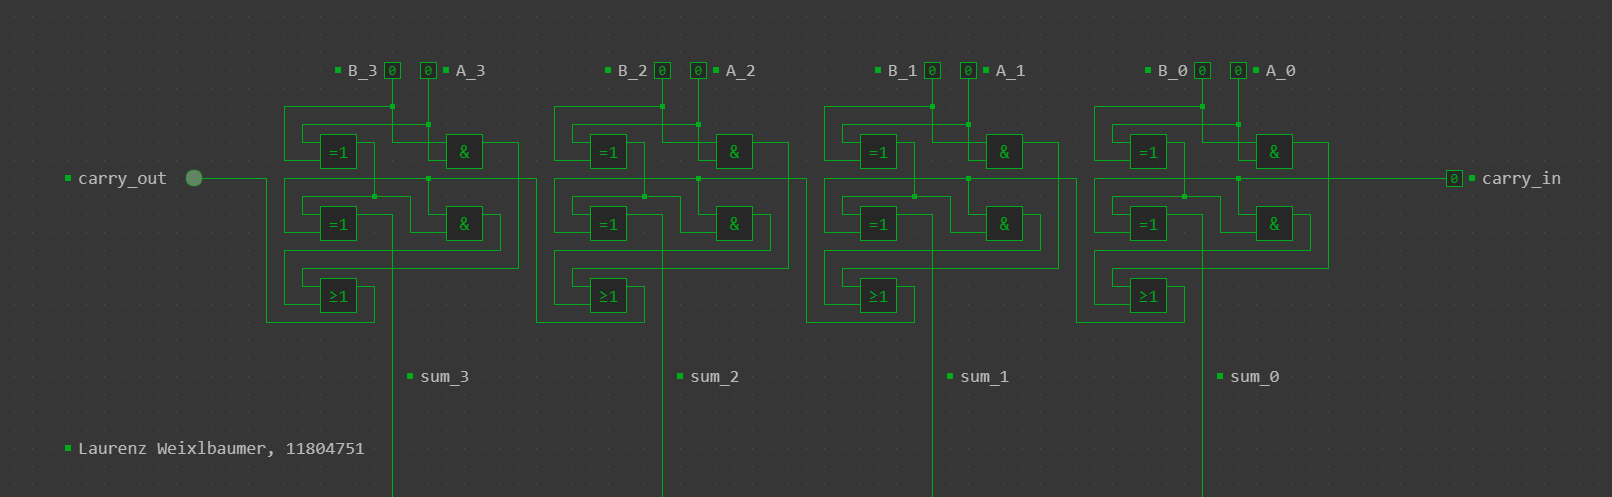
\includegraphics[width=\paperwidth]{adder_circuit.png}}
\end{center}

\item In der gesamten Schaltung sind 20 Gatter zu finden, der längste Pfad beträgt 8 durchlaufene Gatter.

\item Das Ergebnis beträgt $0110_2$, und der carry-out ist $1$ -- ergo ist das tatsächliche Ergebnis $10110_2$.

\end{enumerate}

\end{document}
